\section{Иерархическая система взаимодействующих ostis-сообществ}
{\label{sec_ecosystem_structure}} 

\begin{SCn}


\begin{scnrelfromlist}{ключевое понятие}
    \scnitem{ostis-система}
    \scnitem{самостоятельная ostis-система}
    \scnitem{встроенная ostis-система}
    \scnitem{коллектив ostis-систем}
\end{scnrelfromlist}

\begin{scnrelfromlist}{подраздел}
	\scnitem{\ref{sec_ecosystem_interoperability_support}~\nameref{sec_ecosystem_interoperability_support}}
	\scnitem{\ref{sec_ecosystem_structure_description}~\nameref{sec_ecosystem_structure_description}}
\end{scnrelfromlist}


\bigskip
\begin{scnrelfromlist}{библиографическая ссылка}
	\scnitem{\scncite{Zagorskiy2022a}}
\end{scnrelfromlist}

\end{SCn}

\subsection*{Введение в \ref{sec_ecosystem_structure}}
Для создания успешной \textit{цифровой экосистемы} необходимо решать множество проблем, связанных с обеспечением высокого уровня интероперабельности между самостоятельно действующими системами. Одним из возможных решений является переход к универсальным сообществам индивидуальных \textit{интеллектуальных кибернетических систем}, которые объединяются в \textit{многоагентные системы}.

Реализация такого универсального сообщества интероперабельных \textit{интеллектуальных кибернетических систем} может осуществляться в виде глобальной \textit{Экосистемы OSTIS} (см. \scncite{Zagorskiy2022a}). 
\textit{Экосистема OSTIS} --- социотехническая экосистема, представляющая собой коллектив взаимодействующих \textit{семантических компьютерных систем} и осуществляющая перманентную поддержку эволюции и семантической совместимости всех входящих в нее систем, на протяжении всего их жизненного цикла. 

Система, построенная в соответствии с требованиями и стандартами \textit{Технологии OSTIS}, определяется как \textit{ostis-система}. 

\textit{Экосистема OSTIS} представляет собой коллектив взаимодействующих:
\begin{textitemize}
    \item самих \textit{ostis-систем};
    \item пользователей указанных \textit{ostis-систем} (как конечных пользователей, так и разработчиков);
    \item некоторых \textit{компьютерных систем}, не являющихся \textit{ostis-системами}, но рассматриваемых ими в качестве дополнительных \textit{информационных ресурсов} или \textit{сервисов}.
\end{textitemize}

В рамках \textit{Экосистемы OSTIS} \textit{ostis-системы} способны коммуницировать друг с другом и формировать специализированные коллективы для коллективного решения сложных задач. Такой подход не только повышает уровень интеллекта каждой \textit{индивидуальной кибернетической системы}, но и обеспечивает более эффективное взаимодействие между ними в рамках единой \textit{цифровой экосистемы}. Это обеспечивает существенное развитие целого ряда свойств каждой \textit{компьютерной системы}, позволяющих значительно повысить \textit{уровень интеллекта} (и, прежде всего, их \textit{уровень обучаемости} и \textit{уровень социализации}). 

Участники коллектива \textit{Экосистемы OSTIS} характеризуются как:
\begin{textitemize}
    \item \textit{семантически совместимые};
    \item постоянно эволюционирующие индивидуально;
    \item постоянно поддерживающие свою совместимость с другими участниками в ходе своей индивидуальной эволюции;
    \item способные децентрализованно координировать свою деятельность.
\end{textitemize}

\textit{Экосистема OSTIS} – это переход от \textit{самостоятельных ostis-систем} к \textit{коллективам ostis-систем}, то есть к распределенным \textit{ostis-системам}.

\begin{SCn}
\scnheader{ostis-система}
\begin{scnrelfromset}{разбиение}
    \scnitem{самостоятельная ostis-система}
    \scnitem{встроенная ostis-система}
    \scnitem{коллектив ostis-систем}
\end{scnrelfromset}
\end{SCn}

Цель \textit{Экосистемы OSTIS} --- \myuline{обеспечить постоянную поддержку совместимости компьютерных систем}, входящих в \textit{Экосистему OSTIS} как на этапе их разработки, так и в ходе их эксплуатации. 
Проблема заключается в том, что в ходе эксплуатации систем, входящих в \textit{Экосистему OSTIS}, они могут изменяться из-за чего совместимость может нарушаться. 
\begin{SCn}
    \scnheader{Экосистема OSTIS}
    \begin{scnrelfromlistcustom}{задачи}
        \scnitemcustom{оперативное внедрение всех согласованных изменений стандарта ostis-систем (в том числе, и изменений систем используемых понятий и соответствующих им терминов)}
        \scnitemcustom{перманентная поддержка высокого уровня взаимопонимания всех систем, входящих в \textit{Экосистему OSTIS}, и всех их пользователей}
        \scnitemcustom{корпоративное решение различных комплексных задач, требующих координации деятельности нескольких ostis-систем, а также, возможно, некоторых пользователей}
    \end{scnrelfromlistcustom}
\end{SCn}


\subsection{Поддержка совместимости между ostis-системами, входящими в состав Экосистемы OSTIS}
{\label{sec_ecosystem_interoperability_support}} 

Каждая система, входящая в состав \textit{Экосистемы OSTIS}, должна:
\begin{textitemize}
    \item интенсивно, активно и целенаправленно обучаться, как с помощью учителей-разработчиков, так и самостоятельно;
    \item сообщать всем другим системам о предлагаемых или окончательно утвержденных изменениях в онтологиях и, в частности, в наборе используемых понятий;
    \item принимать от других ostis-систем предложения об изменениях в онтологиях, в том числе в наборе используемых понятий, для согласования или утверждения этих предложений;
    \item реализовывать утвержденные изменения в онтологиях, хранимых в ее базе знаний;
    \item способствовать поддержанию высокого уровня семантической совместимости не только с другими ostis-системами, входящими в \textit{Экосистему OSTIS}, но и со своими пользователями (обучать их, информировать их об изменениях в онтологиях).
\end{textitemize}

К \textit{самостоятельной ostis-системе}, входящей в состав \textit{Экосистемы OSTIS}, предъявляются особые требования:
\begin{textitemize}
    \item она должны обладать всеми необходимыми знаниями и навыками для обмена сообщениями и целенаправленной организации взаимодействия с другими \textit{ostis-системами}, входящими в \textit{Экосистему OSTIS};
    \item в условиях постоянного изменения и эволюции \textit{ostis-систем}, входящих в \textit{Экосистему OSTIS}, она должна сама следить за состоянием своей совместимости (согласованности) со всеми остальными \textit{ostis-системами}, то есть должна самостоятельно поддерживать эту совместимость, согласовывая с другими \textit{ostis-системами} все требующие согласования изменения, происходящие у себя и в других системах.
\end{textitemize}

Для обеспечения высокой эффективности эксплуатации и высоких темпов эволюции \textit{Экосистемы OSTIS} необходимо постоянно повышать уровень информационной совместимости (уровень взаимопонимания) не только между компьютерными системами, входящими в состав \textit{Экосистемы OSTIS}, но также между этими системами и их пользователями. 

Одним из направлений обеспечения такой совместимости является стремление к тому, чтобы база знаний, картина мира каждого пользователя стала частью объединенной базы знаний \textit{Экосистемы OSTIS}. Это значит, что каждый пользователь должен знать, как устроена структура каждой научно-технической дисциплины (объекты исследования, предметы исследования, определения, закономерности и так далее), как могут быть связаны между собой различные дисциплины.

Поддержка совместимости \textit{Экосистемы OSTIS} с ее пользователями осуществляется следующим образом:
\begin{textitemize}
    \item в каждую \textit{ostis-систему} включаются встроенные \textit{ostis-системы}, ориентированные
    \begin{textitemize}
        \item на перманентный мониторинг деятельности конечных пользователей и разработчиков этой \textit{ostis-системы},
        \item на анализ качества и, в первую очередь, корректности этой деятельности,
        \item на повышение квалификации пользователей (персонифицированное обучение);
    \end{textitemize}
    \item в состав \textit{Экосистемы OSTIS} включаются \textit{ostis-системы}, специально предназначенные для обучения пользователей \textit{Экосистемы OSTIS} базовым общепризнанным знаниям и навыкам решения соответствующих классов задач.
\end{textitemize}

\textit{Экосистеме OSTIS} ставится в соответствие ее объединенная база знаний, которая представляет собой виртуальное объединение баз знаний всех ostis-систем, входящих в состав \textit{Экосистемы OSTIS}.
Качество этой базы знаний (полнота, непротиворечивость, чистота) является постоянной заботой всех \textit{самостоятельных ostis-систем}, входящих в состав \textit{Экосистемы OSTIS}.


\subsection{Описание структуры Экосистемы OSTIS}
{\label{sec_ecosystem_structure_description}} 

\begin{SCn}
\begin{scnrelfromlist}{ключевой знак}
    \scnitem{Корпоративная система Экосистемы OSTIS}
\end{scnrelfromlist}

\begin{scnrelfromlist}{ключевое понятие}
    \scnitem{агент Экосистемы OSTIS}
    \scnitem{пользователь Экосистемы OSTIS}
    \scnitem{ostis-сообщество}
\end{scnrelfromlist}
\end{SCn}

Субъект, входящий в состав \textit{Экосистемы OSTIS}, является \textit{агентом Экосистемы OSTIS}.

\begin{SCn}
\scnheader{агент Экосистемы OSTIS}
\begin{scnrelfromset}{разбиение}
    \scnitem{индивидуальная ostis-система Экосистемы OSTIS}
	\begin{scnindent}
    \begin{scnrelfromset}{разбиение}
        \scnitem{самостоятельная ostis-система Экосистемы OSTIS}
        \scnitem{встроенная ostis-система Экосистемы OSTIS}
    \end{scnrelfromset}
	\end{scnindent}
    \scnitem{пользователь Экосистемы OSTIS}
    \scnitem{ostis-сообщество}
	\begin{scnindent}
    \begin{scnrelfromset}{разбиение}
        \scnitem{простое ostis-сообщество}
        \scnitem{иерархическое ostis-сообщество}
    \end{scnrelfromset}
	\end{scnindent}
\end{scnrelfromset}
\end{SCn}

Понятие \textit{ostis-сообщества} представляет собой не только \textit{коллектив ostis-систем}, но также определенный коллектив людей (пользователей и разработчиков соответствующих \textit{ostis-систем}). 
\textit{ostis-сообщество} является устойчивым фрагментом \textit{Экосистемы OSTIS}, обеспечивающим комплексную автоматизацию определенной части коллективной человеческой деятельности и перманентное повышение ее эффективности. 
\textit{иерархическим ostis-сообществом} называется такое \textit{ostis-сообщество}, по крайней мере одним из членов которого является некоторое другое \textit{ostis-сообщество}.

Правила поведения \textit{агентов Экосистемы OSTIS}:
\begin{textitemize}
    \item согласовывать денотационную семантику всех используемых знаков (в первую очередь понятий);
    \item согласовывать терминологию, устранять противоречия и информационные дыры;
    \item постоянно бороться с синонимией и омонимией как на уровне sc-элементов (внутренних знаков), так и на уровне соответствующих им терминов и прочих внешних идентификаторов (внешних обозначений);
    \item каждый \textit{агент Экосистемы OSTIS} по своей инициативе может стать членом любого ostis-сообщества Экосистемы OSTIS после соответствующей регистрации;
\end{textitemize}

Все правила поведения \textit{агентов Экосистемы OSTIS} должны соблюдаться не только \textit{ostis-системами}, которые являются агентами \textit{Экосистемы OSTIS}, но и людьми, являющиеся ими. 
Корректное поведение \textit{ostis-систем} как \textit{агентов Экосистемы OSTIS} значительно проще обеспечить, чем корректное поведение людей в качестве таких агентов. 
Поведение пользователей (естественных агентов) \textit{Экосистемы OSTIS} необходимо внимательно мониторить и контролировать, постоянно способствуя повышению уровня их квалификации как \textit{агентов Экосистемы OSTIS}, а также повышению уровня их мотивации, целенаправленности и самореализации.

\textit{Экосистема OSTIS} является максимальным \textit{иерархическим ostis-сообществом}, обеспечивающим комплексную автоматизацию всех видов человеческой деятельности. 
Оно не может входить в состав какого-либо другого \textit{ostis-сообщества}. 
Принципы, лежащие в основе \textit{Экосистемы OSTIS}:
\begin{textitemize}
    \item \textit{Экосистема OSTIS} представляет собой сеть \textit{ostis-сообществ};
    \item Каждому \textit{ostis-сообществу} взаимно однозначно соответствует \textit{корпоративная ostis-система} этого \textit{ostis-сообщества};
    \item Каждое \textit{ostis-сообщество} может входить в состав любого другого \textit{ostis-сообщества} по своей инициативе. Формально это означает, что \textit{корпоративная ostis-система} первого \textit{ostis-сообщества} является членом другого \textit{ostis-сообщества};
    \item Каждому специалисту, входящему в состав \textit{Экосистемы OSTIS} ставится во взаимнооднозначное соответствие его \textit{персональный ostis-ассистент}, который трактуется как \textit{корпоративная ostis-система} вырожденного \textit{ostis-сообщества}, состоящего из одного человека.
\end{textitemize}

В \textit{Экосистеме OSTIS} можно выделить следующие уровни иерархии:
\begin{textitemize}
    \item индивидуальные \textit{кибернетические системы} (индивидуальные \textit{ostis-системы} и люди, являющиеся конечными пользователями \textit{ostis-систем});
    \item иерархическая система \textit{ostis-сообществ}, членами каждого из которых могут быть \textit{индивидуальные ostis-системы}, люди, а также другие \textit{ostis-сообщества};
    \item \textit{Максимальное ostis-сообщество} \textit{Экосистемы OSTIS}, не являющееся членом никакого другого \textit{ostis-сообщества}, входящего в состав \textit{Экосистемы OSTIS}.
\end{textitemize}

Качество \textit{Экосистемы OSTIS} во многом определяется эффективностью взаимодействия каждой \textit{ostis-системы} (в том числе каждого \textit{ostis-сообщества}), каждого человека со своей внешней средой, а также качеством и чистотой самой внешней среды. 
Потому основной целью \textit{Экосистемы OSTIS} является повышение качества информационной внешней среды для всех субъектов, входящих в состав \textit{Экосистемы OSTIS}.
Иными словами, \textit{Экосистема OSTIS} обеспечивает поддержку информационной экологии человеческого общества.

\begin{SCn}
\scnheader{ostis-сообщество}
\begin{scnrelfromset}{разбиение}
    \scnitem{минимальное ostis-сообщество}
    \scnitem{коллектив ostis-систем}
\end{scnrelfromset}
\end{SCn}

Каждой персоне, входящей в состав \textit{Экосистемы OSTIS} взаимно однозначно соответствует его личный (персональный) ассистент в виде \textit{персонального ostis-ассистента}.
Таким образом, количество \textit{персональных ostis-ассистентов}, входящих в состав \textit{Экосистемы OSTIS}, совпадает с числом персон, входящих в состав \textit{Экосистемы OSTIS} (см. \nameref{fig:ostis_assistant}).

\begin{figure}[H]
    \caption{SCg-текст. Пример \textit{персоны} и соответствующего ему \textit{персонального ostis-ассистента}}
    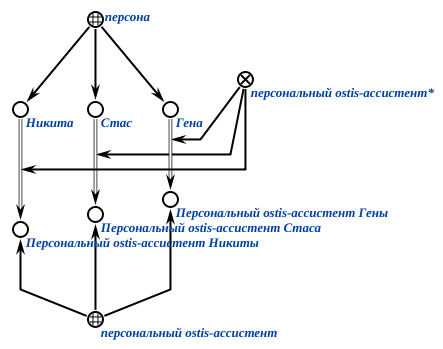
\includegraphics[scale=0.8]{author/part7/chapter_ecosystem/figures/personal_ostis_assistant_example_ru.png}
    \label{fig:ostis_assistant}
\end{figure}

Коллектив, состоящий из персоны и соответствующего ей \textit{персонального ostis-ассистента}, фактически является \textit{минимальным ostis-сообществом}(см. \nameref{fig:ostis_corporate}).

\begin{figure}[H]
    \caption{SCg-текст. Пример \textit{минимального ostis-сообщества}}
    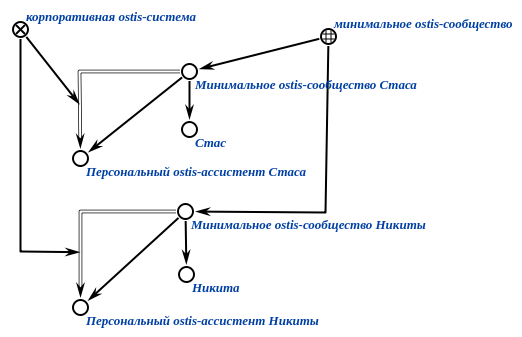
\includegraphics[scale=0.8]{author/part7/chapter_ecosystem/figures/corporate_ostis_system_example_ru.png}
    \label{fig:ostis_corporate}
\end{figure}

Поскольку формально в не \textit{минимальные ostis-сообщества} входят не персоны, а соответствующие им \textit{персональные ostis-ассистенты}, все \textit{ostis-сообщества}, кроме \textit{минимальных ostis-сообществ}, являются \textit{коллективами ostis-систем}.

\textit{корпоративная ostis-система} есть центральная \textit{ostis-система}, осуществляющая координацию, организацию, а также поддержку эволюции деятельности членов соответствующего \textit{ostis-сообщества}. 
\textit{корпоративная ostis-система} является представителем соответствующего \textit{ostis-сообщества} в других \textit{ostis-сообществах}, членом которых оно является(см. \nameref{fig:ostis_community}).

\begin{figure}[H]
    \caption{SCg-текст. Пример \textit{корпоративной ostis-системы} \textit{ostis-сообщества}}
    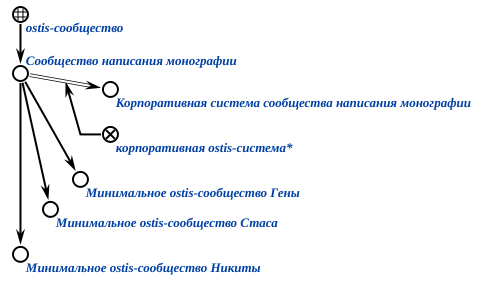
\includegraphics[scale=0.8]{author/part7/chapter_ecosystem/figures/ostis-system collectivity_example_ru.png}
    \label{fig:ostis_community}
\end{figure}

Основным назначением \textit{Корпоративной системы Экосистемы OSTIS} является организация общего взаимодействия при выполнении самых различных видов и областей человеческой деятельности, которые могут быть либо полностью автоматизированными, либо частично автоматизированными, либо вообще неавтоматизированными. 
Из этого следует, что база знаний \textit{Корпоративной системы Экосистемы OSTIS} должна содержать \textit{Общую формальную теорию человеческой деятельности}, включающей в себя типологию видов и областей человеческой деятельности, а также общую методологию этой деятельности.

\begin{SCn}
\scnheader{Деятельность в области Искусственного интеллекта, осуществляемая на основе Технологии OSTIS}
\scnrelfrom{основной продукт}{Экосистема OSTIS}
\begin{scnrelfromlist}{подпроект}
    \scnitem{Проект Метасистемы OSTIS}
    \scnitem{Проект программной реализации абстрактной sc-машины}
    \scnitem{Проект разработки универсального sc-компьютера}
\end{scnrelfromlist}
\end{SCn}

Продуктом человеческой деятельности в области Искусственного интеллекта, осуществляемой на основе \textit{Технологии OSTIS}, является не просто множество \textit{ostis-систем} различного назначения, а Экосистема, состоящая из взаимодействующих \textit{ostis-систем} и их пользователей. 

По назначению \textit{ostis-системы}, входящие в \textit{Экосистему OSTIS}, могут быть:
\begin{textitemize}
    \item ассистентами конкретных пользователей или конкретных пользовательских коллективов;
    \item типовыми встраиваемыми подсистемами \textit{ostis-систем};
    \item системами информационной и инструментальной поддержки проектирования различных компонентов и различных классов \textit{ostis-систем};
    \item системами информационной и инструментальной поддержки проектирования или производства различных классов технических и других искусственно создаваемых систем;
    \item порталами знаний по самым различным научным дисциплинам;
    \item системами автоматизации управления различными сложными объектами (производственными предприятиями, учебными заведениями, кафедрами вузов, конкретными обучаемыми);
    \item интеллектуальными справочными и help-системами;
    \item интеллектуальными робототехническими системами.
\end{textitemize}
Типология \textit{ostis-систем}, являющихся агентом Экосистемы OSTIS, представлена ниже.

\begin{SCn}
\scnheader{ostis-система, являющаяся агентом Экосистемы OSTIS}
\scnsuperset{персональный ostis-ассистент}
\scnsuperset{корпоративная ostis-система}
\scnsuperset{ostis-портал знаний}
\scnsuperset{ostis-система автоматизации проектирования}
\scnsuperset{ostis-система автоматизации производства}
\scnsuperset{ostis-система автоматизации образовательной деятельности}
\begin{scnindent}
	\scnsuperset{обучающаяся ostis-система}
	\scnsuperset{корпоративная ostis-система виртуальной кафедры}
\end{scnindent}
\scnsuperset{ostis-система автоматизации бизнес-деятельности}
\scnsuperset{ostis-система автоматизации управления}
\begin{scnindent}
	\scnsuperset{ostis-система управления проектами соответствующего вида}
	\scnsuperset{ostis-система сенсомоторной координации при выполнении определенного вида сложных действий во внешней среде}
    \begin{scnindent}
        \scnsuperset{ostis-система управления самостоятельным перемещением} 
		\scnsuperset{робота по пересеченной местности}
    \end{scnindent}
\end{scnindent}
\end{SCn}
